\documentclass[12pt,a4paper]{article}
\usepackage[top=2.5cm,bottom=2.5cm,left=2.2cm,right=2.2cm]{geometry}
\usepackage{polski}
\usepackage[utf8]{inputenc}
%%\usepackage[OT4]{fontenc}
\usepackage{amsmath,amsfonts,amssymb,amsthm}
\usepackage{enumerate}
\usepackage{url}
\usepackage{multicol}
\usepackage{color}
\usepackage{graphicx} 
\usepackage{setspace}
\usepackage{float}
\usepackage{subfig}
\usepackage{listings}
\usepackage{pythonhighlight}
\usepackage{lipsum}
\usepackage{tabularx}
\usepackage{hyperref}

%\pagestyle{empty}
%WYMIARY STRONY
\topmargin -30mm
\oddsidemargin -1.7cm
\evensidemargin -1.7cm
\textwidth 180mm
\textheight 260mm
%\usepackage{psfrag}

\usepackage{amsmath}
\usepackage{amsfonts}

\usepackage{supertabular}
\usepackage{array}


\usepackage{tabularx}
\usepackage{hhline}

\newcommand{\myand}{i\ }
%\usepackage{showlabels}

\newcommand{\R}{I\!\!R} %symbol liczb rzeczywistych, dzia³a tylko w
                        %trybie matematycznym
\newtheorem{theorem}{Twierdzenie}[section] %nowe otoczenie do
                                           %sk³adania twierdzeñ

\usepackage{titlesec}
\titleformat*{\section}{\normalsize\bfseries}
\titleformat*{\subsection}{\footnotesize\bfseries}
\titleformat*{\subsubsection}{\normalsize}
\title{Wybrane metody klasteryzacji w oparciu o system R}
\date{24.04.2018}
\author{Łukasz Odwrot 218283}

%ustawianie marginesów
\usepackage{geometry}
\newgeometry{tmargin=2.5cm, bmargin=2.5cm, lmargin=2.5cm, rmargin=2.5cm}


 
 
\begin{document}
\maketitle
\thispagestyle{empty}
\newpage
\tableofcontents
\setcounter{page}{1}
\newpage

\section{Wstęp}
Klasteryzacja to forma nienadzorowanego uczenia. Polega ona na przypisaniu obiektów ze zbioru na podstawie podobieństwa cech do klastrów, których ilość zwykle jest parametrem wejściowym algorytmu klasteryzacji.
\section{Badane zbiory}

Klasteryzacja badana będzie na 4 zbiorach.
\begin{figure}[H]
\centering
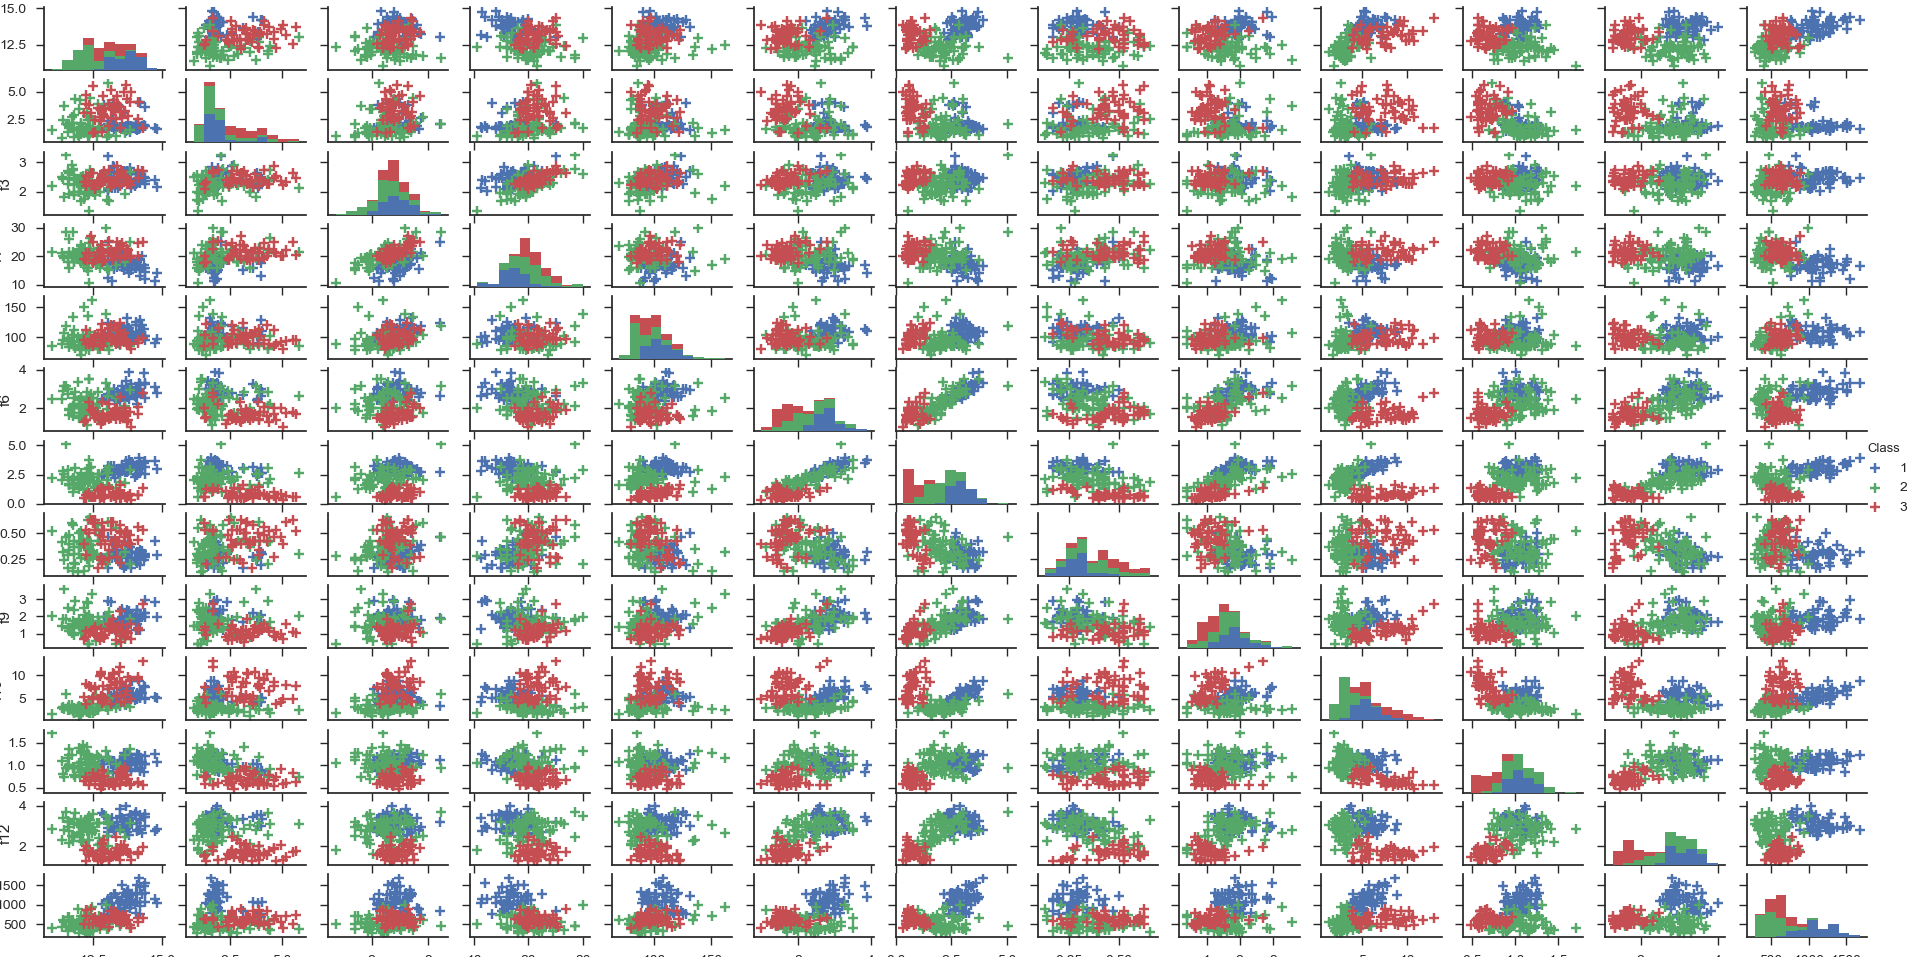
\includegraphics[width=1\textwidth]{dsWineCombined.png}
\caption{Rozkład cech dla zbioru Wine}
\end{figure}

\begin{figure}[H]
\centering
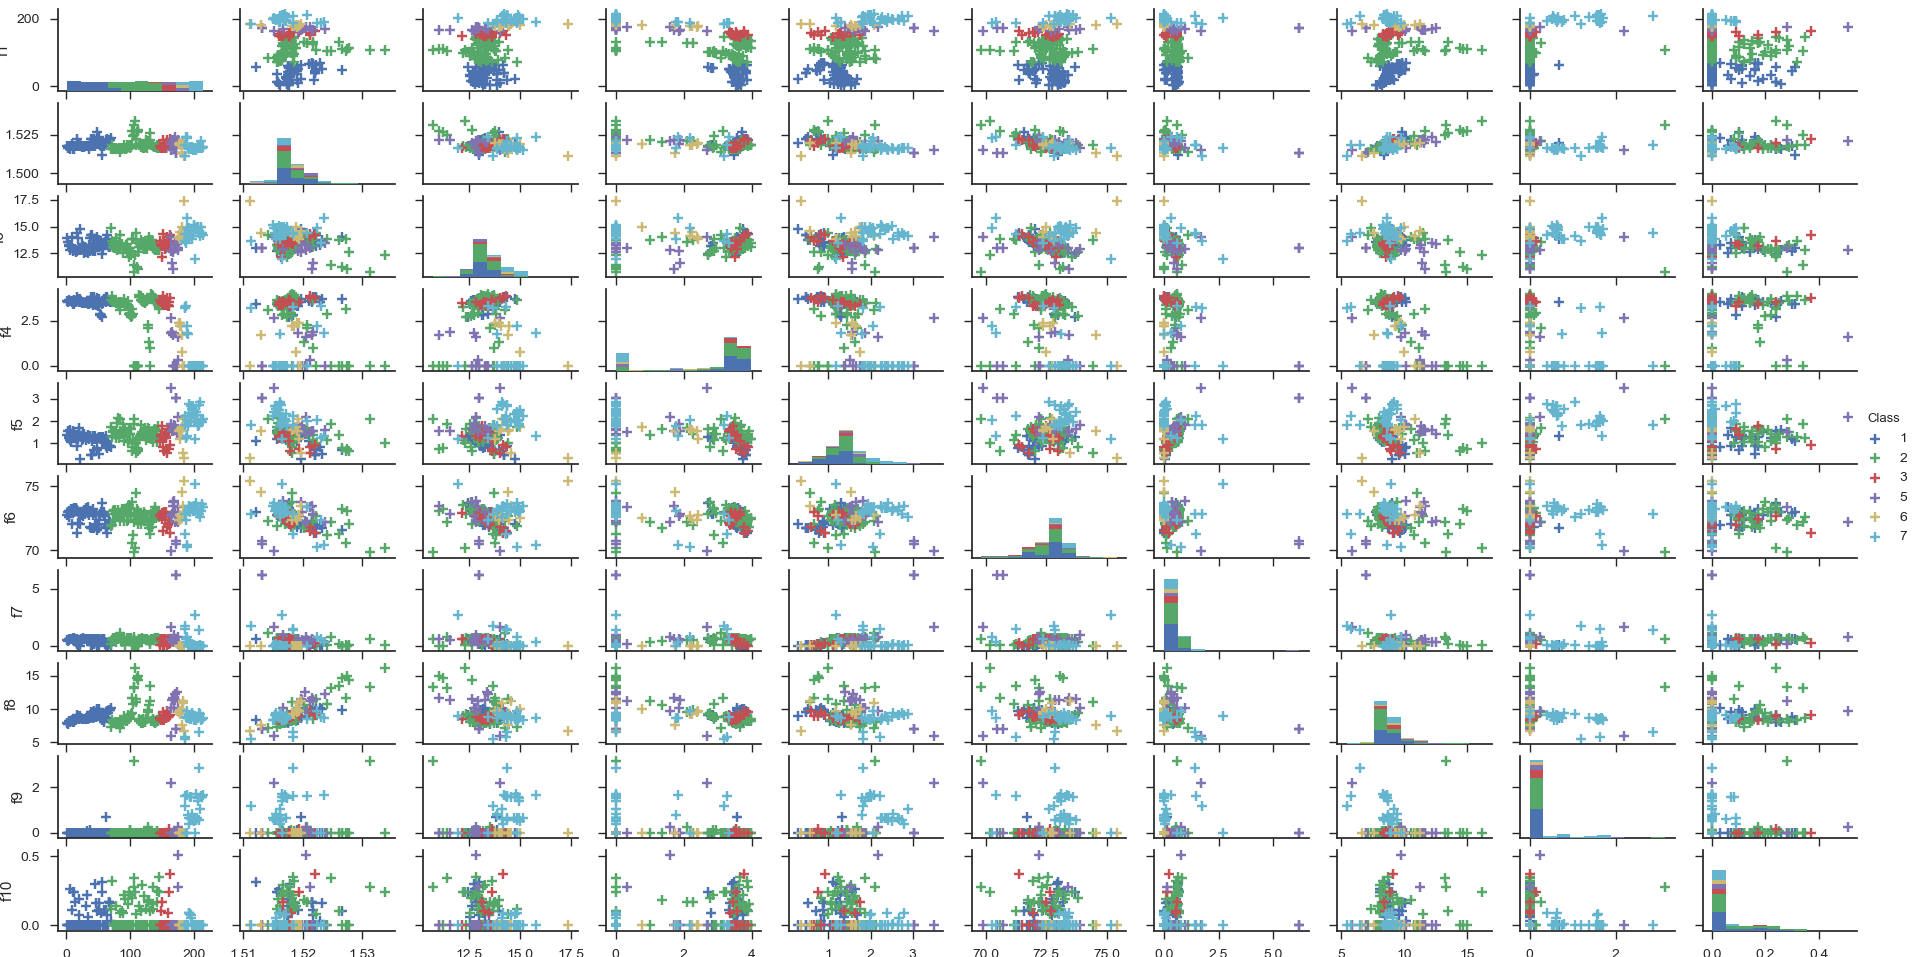
\includegraphics[width=1\textwidth]{dsGlassCombined.png}
\caption{Rozkład cech dla zbioru Glass}
\end{figure}

\begin{figure}[H]
\centering
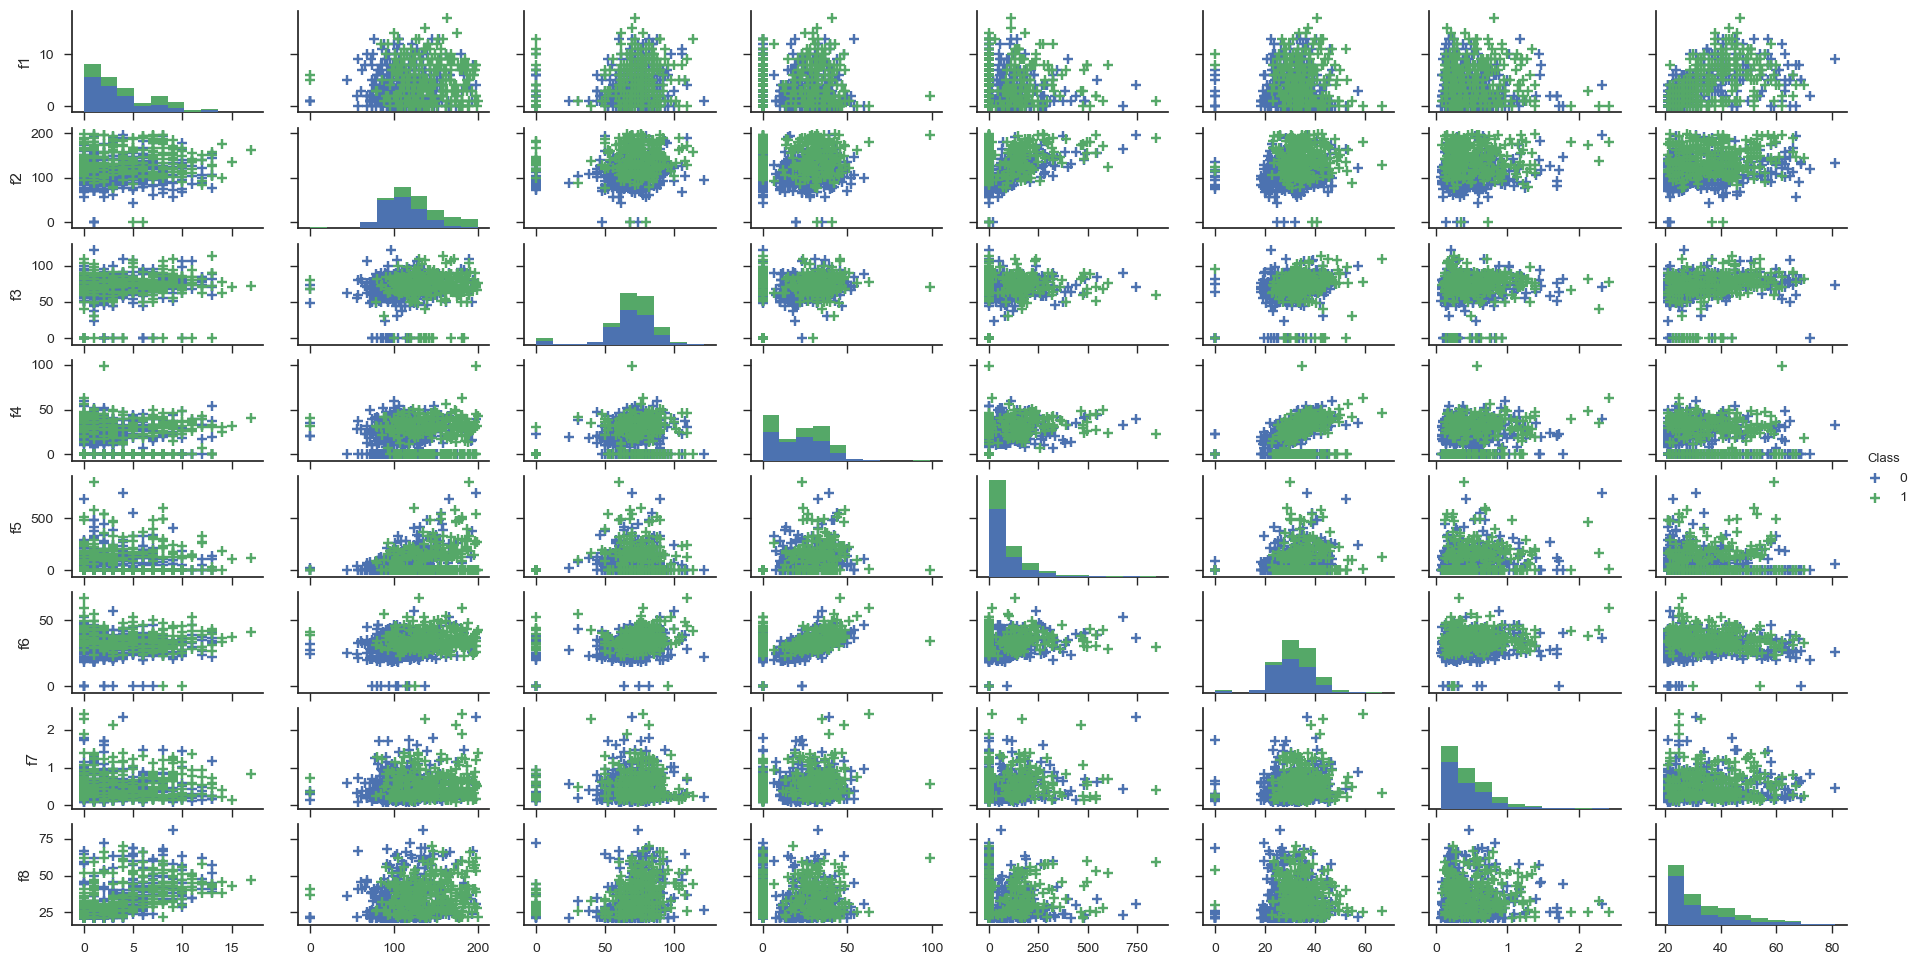
\includegraphics[width=1\textwidth]{dsDiabetesCombined.png}
\caption{Rozkład cech dla zbioru Diabetes}
\end{figure}

\begin{figure}[H]
\centering
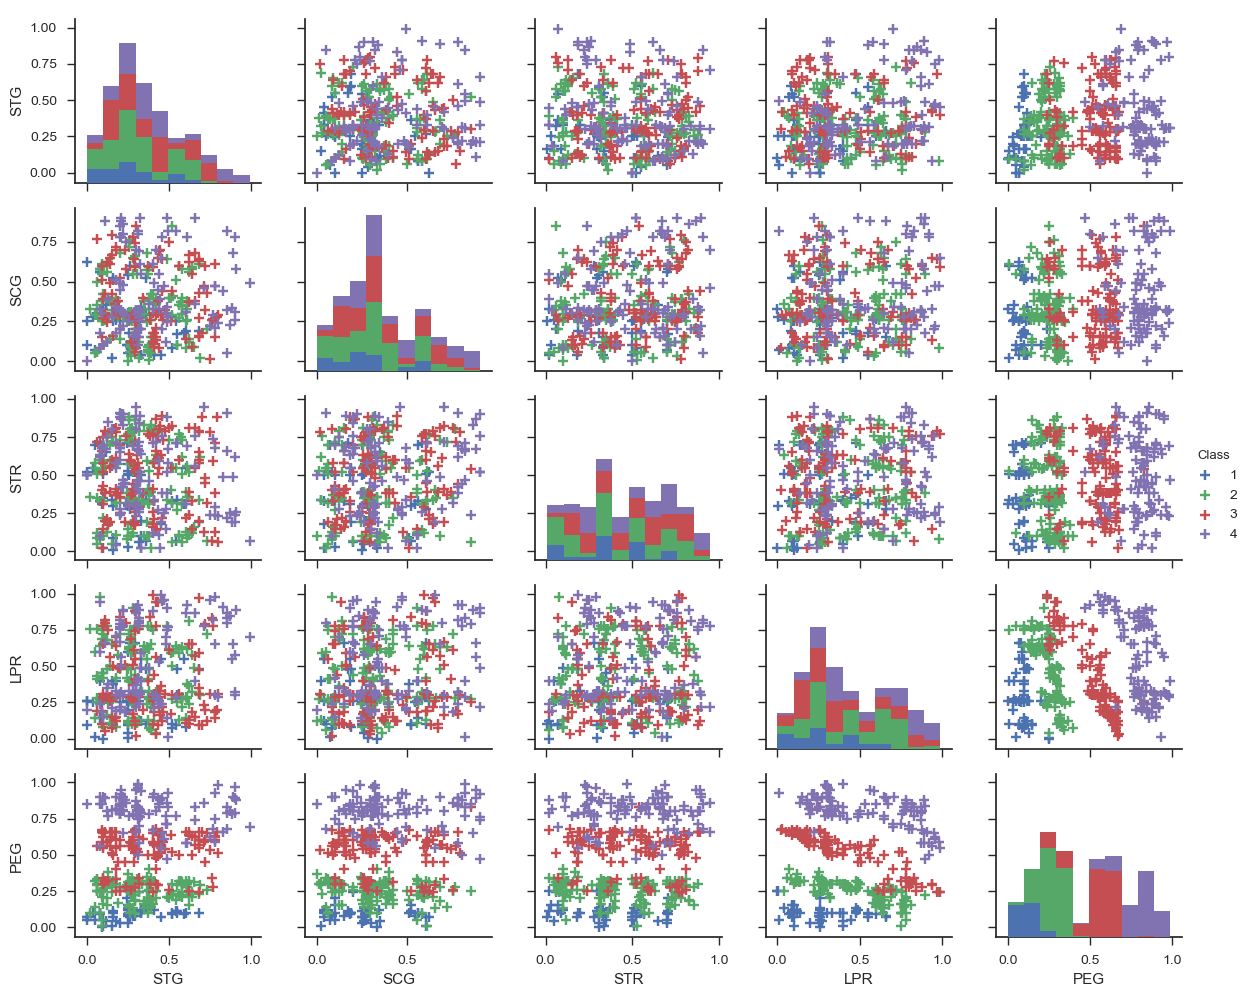
\includegraphics[width=1\textwidth]{dsKnowledgeCombined.png}
\caption{Rozkład cech dla zbioru Knowledge}
\end{figure}


\section{Metody klasteryzacji}
Zbadane zostaną dwie metody klasteryzacji.\\
\textbf{K-means}\\
Metoda ta polega na przyporządkowaniu danych wejściowych, w których każda próbka należy do klastra z najbliższą wartością średnią. Każda próbka to wielowymiarowy wektor liczb rzeczywistych.\\
Na wejściu algorytmu podawane są parametry : \\
k - ilość klastrów\\
data - dane wejściowe\\
Algorytm działa następująco:\\
1. Rozmieszcza centroidy  w losowych miejscach przestrzeni, \\
2. Dla każdego punktu znajduje najbliższą centroidę i przypisuje punkt do centroidy,\\
3. Na podstawie wszystkich próbek przypisanych do centroidy wyliczane są wartości średnie i powtarzany jest krok 2 dopóki warunki stopu nie zostaną spełnione lub nie nie zmieniło się przypisanie próbek.\\
Metoda przeznaczona jest jedynie dla danych numerycznych.\\
W funkcji klasteryzacji kmeans w R możemy zdefiniować maksymalną liczbę iteracji (domyślnie 10) oraz ilość losowań początkowych pozycji, z których wybrana zostanie najlepsza.\\
\textbf{Partitioning Around Medoids}\\
Używa ona zachłannego algorytmu, więc może nie znaleźć najlepszego rozwiązania, ale dzięki temu jest relatywnie szybka. Działa według następującego schematu.\\
1. Wybiera k reprezentatów, które będą centami klastrów.
2. Przypisuje wszystkie punkty do najbliższego klastra.
3. Dla każdej próbki będącą centrum medoidy i dla każdej próbki nie będącej centrum zamień je. Jeżeli konfiguracja pogorszyła się, cofnij zmianę.\\
Koszt wyliczany jest jako suma odległości próbek w klastrze od jego centrum.


\section{Ocena klasteryzacji}
Do oceny jakości klasteryzacji posłużą nam następujące miary:\\
\textbf{Purity}\\
Informuje w jakim stopniu klastry odpowiadają pojedynczym klasom. Warto zaznaczyć, że w przypadku takiej samej ilości klas co klastrów funkcja zawsze zwróci wartość 1.

$$ \frac{1}{N} = \sum_{m \in M} \max_{d \in D} | m \cap d |   $$

\textbf{Rand measure}
Porównuje jak podobne są klastry względem wzorca. Miara może być interpretowana jako procentowa ilość podjętych prawidłowych decyzji.

$$ RI = \frac{TP + TN}{TP + FP + FN + TN}$$

\textbf{Dunn index}
Miara ta odzwierciedla gęstość i poprawność odseparowania klastrów. Wyliczana jest na podstawie stosunku minimalnej odległości wewnątrz klastra do maksymalnej odległości wewnątrz klastra.

\textbf{Davies–Bouldin index}
Miarę tę można obliczyć na podstawie poniższego wzoru.

$$ DB = \frac{1}{n} \sum_{i=1}^{n} \max{(\frac{\sigma _{i} + \sigma _{j}}{d(c_i, c_j)})}   $$

Gdzie n jest liczbą klastrów, c - centroidą klastra, $ \sigma $ - średnia odległość od wszystkich elementów klastra. Algorytm dające niskie odległości wewnątrz klastra i duże odległości między klastrami będą dawały niskie wyniki.

\section{Klasteryzacja zbiorów}
\begin{tabular}{ |p{1.5cm}||p{2.5cm}|p{2.5cm}|p{2.5cm}|p{2.5cm}| }
\hline
\multicolumn{5}{|c|}{Instanacja Wine}\\
\hline
k &Purity & Rand Index & Dann Index & DBI \\
\hline
\hline
\multicolumn{5}{|c|}{Kmean}\\
\hline
2 & 0.601 & 0.681 & 0.168 & 1.404\\
3 & 0.955 & 0.941 & 0.189 & 1.370\\
4 & 0.966 & 0.895 & 0.186 & 1.793\\
6 & 0.949 & 0.822 & 0.192 & 1.867\\
10 & 0.955 & 0.770 & 0.174 & 1.739\\
15 & 0.983 & 0.741 & 0.261 & 1.599\\
20 & 0.949 & 0.713 & 0.286 & 1.581\\
30 & 0.978 & 0.702 & 0.290 & 1.344\\
50 & 0.978 & 0.681 & 0.332 & 1.155\\
75 & 0.994 & 0.673 & 0.437 & 0.945\\
100 & 1.000 & 0.669 & 0.500 & 0.728\\
\hline
\multicolumn{5}{|c|}{Pam Stats}\\
\hline
2 & 0.601 & 0.679 & 0.168 & 1.422\\
3 & 0.904 & 0.878 & 0.229 & 1.408\\
4 & 0.904 & 0.845 & 0.173 & 2.091\\
6 & 0.961 & 0.814 & 0.199 & 2.090\\
10 & 0.944 & 0.747 & 0.167 & 2.067\\
15 & 0.933 & 0.724 & 0.188 & 1.814\\
20 & 0.938 & 0.714 & 0.235 & 1.655\\
30 & 0.961 & 0.699 & 0.284 & 1.357\\
50 & 0.983 & 0.686 & 0.320 & 1.084\\
75 & 0.994 & 0.676 & 0.414 & 0.883\\
100 & 1.000 & 0.672 & 0.482 & 0.672\\
\hline
\end{tabular}

\begin{tabular}{ |p{1.5cm}||p{2.5cm}|p{2.5cm}|p{2.5cm}|p{2.5cm}| }
\hline
\multicolumn{5}{|c|}{Instanacja Glass}\\
\hline
k &Purity & Rand Index & Dann Index & DBI \\
\hline
\hline
\multicolumn{5}{|c|}{Kmean}\\
\hline
2 & 0.444 & 0.549 & 0.064 & 1.186\\
3 & 0.495 & 0.586 & 0.112 & 1.401\\
4 & 0.519 & 0.631 & 0.049 & 1.403\\
6 & 0.547 & 0.667 & 0.045 & 1.181\\
10 & 0.575 & 0.703 & 0.066 & 1.141\\
15 & 0.673 & 0.745 & 0.052 & 1.156\\
20 & 0.692 & 0.746 & 0.048 & 1.079\\
30 & 0.715 & 0.746 & 0.057 & 0.977\\
50 & 0.794 & 0.751 & 0.069 & 0.858\\
75 & 0.846 & 0.747 & 0.089 & 0.703\\
100 & 0.869 & 0.744 & 0.085 & 0.615\\
\hline
\multicolumn{5}{|c|}{Pam Stats}\\
\hline
2 & 0.444 & 0.538 & 0.137 & 1.174\\
3 & 0.467 & 0.615 & 0.032 & 1.438\\
4 & 0.514 & 0.635 & 0.043 & 1.409\\
6 & 0.528 & 0.661 & 0.035 & 1.534\\
10 & 0.659 & 0.741 & 0.023 & 1.535\\
15 & 0.682 & 0.747 & 0.039 & 1.244\\
20 & 0.710 & 0.749 & 0.033 & 1.071\\
30 & 0.752 & 0.757 & 0.066 & 0.876\\
50 & 0.804 & 0.750 & 0.088 & 0.710\\
75 & 0.836 & 0.749 & 0.157 & 0.570\\
100 & 0.874 & 0.745 & 0.201 & 0.470\\
\hline
\end{tabular}

\begin{tabular}{ |p{1.5cm}||p{2.5cm}|p{2.5cm}|p{2.5cm}|p{2.5cm}| }
\hline
\multicolumn{5}{|c|}{Instanacja Diabetes}\\
\hline
k &Purity & Rand Index & Dann Index & DBI \\
\hline
\hline
\multicolumn{5}{|c|}{Kmean}\\
\hline
2 & 0.668 & 0.556 & 0.072 & 1.721\\
3 & 0.667 & 0.538 & 0.066 & 1.842\\
4 & 0.660 & 0.546 & 0.066 & 1.614\\
6 & 0.704 & 0.531 & 0.050 & 1.753\\
10 & 0.708 & 0.504 & 0.071 & 1.663\\
15 & 0.715 & 0.485 & 0.067 & 1.598\\
20 & 0.736 & 0.485 & 0.075 & 1.563\\
30 & 0.754 & 0.471 & 0.062 & 1.634\\
50 & 0.768 & 0.465 & 0.068 & 1.449\\
75 & 0.776 & 0.462 & 0.114 & 1.392\\
100 & 0.790 & 0.460 & 0.103 & 1.306\\
\hline
\multicolumn{5}{|c|}{Pam Stats}\\
\hline
2 & 0.665 & 0.554 & 0.076 & 1.730\\
3 & 0.651 & 0.524 & 0.055 & 1.945\\
4 & 0.663 & 0.537 & 0.034 & 2.008\\
6 & 0.672 & 0.514 & 0.034 & 1.995\\
10 & 0.694 & 0.489 & 0.068 & 1.812\\
15 & 0.721 & 0.480 & 0.051 & 1.785\\
20 & 0.729 & 0.474 & 0.068 & 1.753\\
30 & 0.743 & 0.468 & 0.069 & 1.739\\
50 & 0.762 & 0.464 & 0.085 & 1.613\\
75 & 0.779 & 0.462 & 0.116 & 1.434\\
100 & 0.792 & 0.460 & 0.123 & 1.357\\
\hline
\end{tabular}

\begin{tabular}{ |p{1.5cm}||p{2.5cm}|p{2.5cm}|p{2.5cm}|p{2.5cm}| }

\hline
\multicolumn{5}{|c|}{Instanacja Knowledge}\\
\hline
k &Purity & Rand Index & Dann Index & DBI \\
\hline
\hline
\multicolumn{5}{|c|}{Kmean}\\
\hline
2 & 0.572 & 0.694 & 0.107 & 1.966\\
3 & 0.557 & 0.687 & 0.072 & 1.720\\
4 & 0.622 & 0.716 & 0.082 & 1.671\\
6 & 0.592 & 0.717 & 0.105 & 1.459\\
10 & 0.632 & 0.729 & 0.082 & 1.406\\
15 & 0.667 & 0.735 & 0.122 & 1.320\\
20 & 0.654 & 0.731 & 0.117 & 1.248\\
30 & 0.759 & 0.736 & 0.155 & 1.262\\
50 & 0.816 & 0.736 & 0.161 & 1.211\\
75 & 0.848 & 0.734 & 0.173 & 1.114\\
100 & 0.871 & 0.732 & 0.178 & 1.040\\
\hline
\multicolumn{5}{|c|}{Pam Stats}\\
\hline
2 & 0.478 & 0.594 & 0.056 & 2.057\\
3 & 0.463 & 0.643 & 0.059 & 1.745\\
4 & 0.505 & 0.663 & 0.079 & 1.695\\
6 & 0.550 & 0.709 & 0.075 & 1.515\\
10 & 0.652 & 0.729 & 0.090 & 1.396\\
15 & 0.697 & 0.734 & 0.093 & 1.449\\
20 & 0.716 & 0.737 & 0.111 & 1.419\\
30 & 0.774 & 0.739 & 0.125 & 1.346\\
50 & 0.838 & 0.737 & 0.125 & 1.270\\
75 & 0.871 & 0.735 & 0.159 & 1.199\\
100 & 0.888 & 0.734 & 0.265 & 1.045\\
\hline
\end{tabular}


\section{Wizualizacja klasteryzacji}
Na przykładzie zbioru Diabetes zostanie zwizualizowane przyporządkowanie próbek do poszczególnych klastrów.

\begin{figure}[H]
\centering
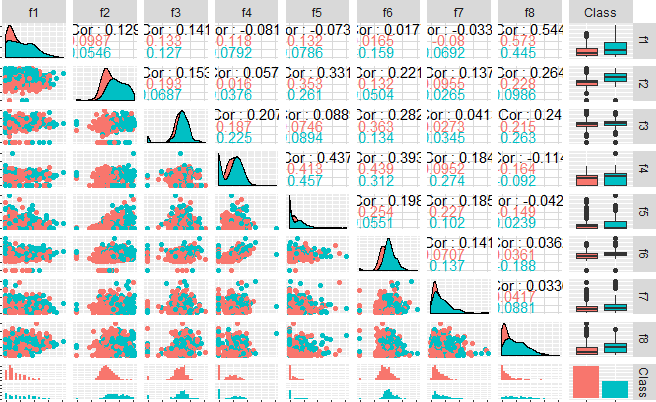
\includegraphics[width=1\textwidth]{diabetesClasses.PNG}
\caption{Rozkład klas dla instancji Diabetes}
\end{figure}

Metoda klasteryzacji kmean Dla zbioru Diabetes.

\begin{figure}[H]
\centering
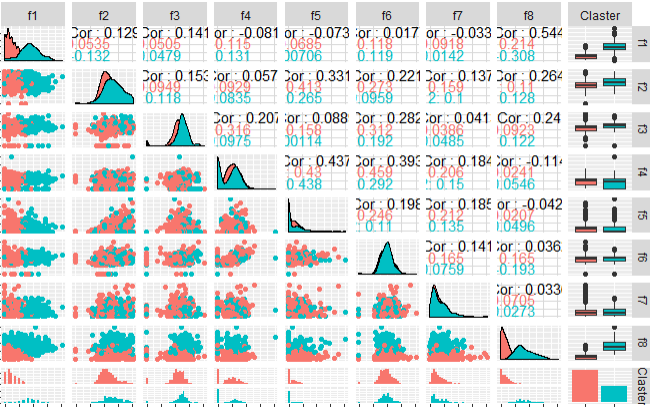
\includegraphics[width=1\textwidth]{diabetesK2.PNG}
\caption{Podział na dwa klastry}
\end{figure}

\begin{figure}[H]
\centering
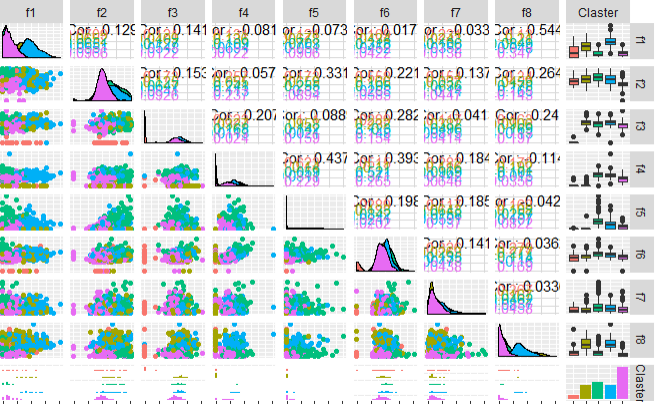
\includegraphics[width=1\textwidth]{diabetesK5.PNG}
\caption{Podział na pięć klastrów}
\end{figure}

\begin{figure}[H]
\centering
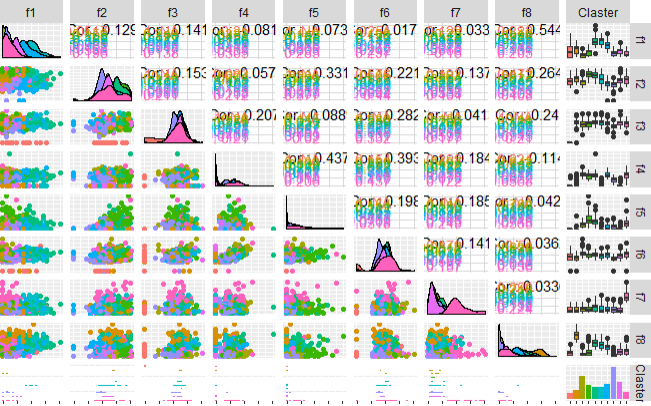
\includegraphics[width=1\textwidth]{diabetesK10.PNG}
\caption{Podział na dziesięć klastrów}
\end{figure}

Metoda klasteryzacji Partitioning Around Medoids Dla zbioru Diabetes.

\begin{figure}[H]
\centering
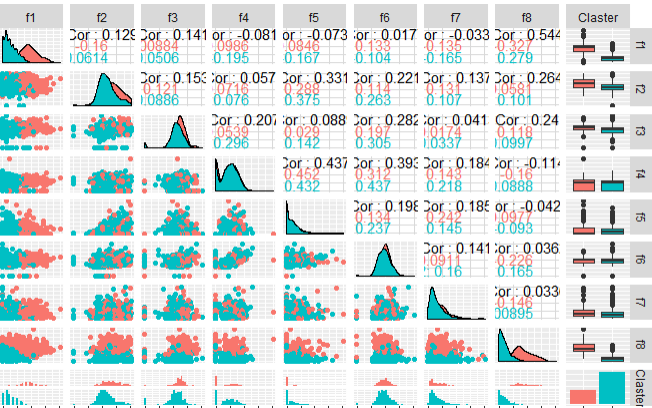
\includegraphics[width=1\textwidth]{diabetesP2.PNG}
\caption{Podział na dwa klastry}
\end{figure}

\begin{figure}[H]
\centering
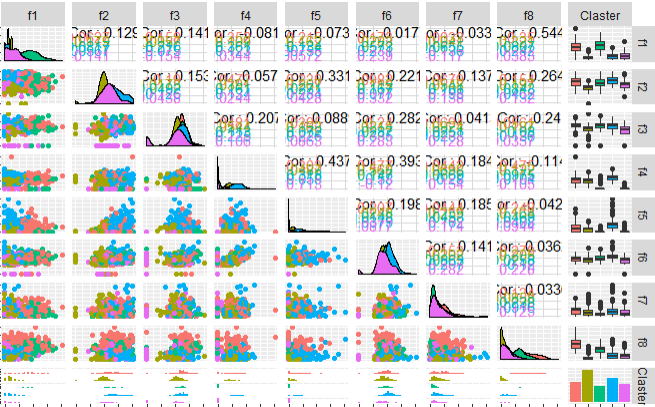
\includegraphics[width=1\textwidth]{diabetesP5.PNG}
\caption{Podział na pięć klastrów}
\end{figure}

\begin{figure}[H]
\centering
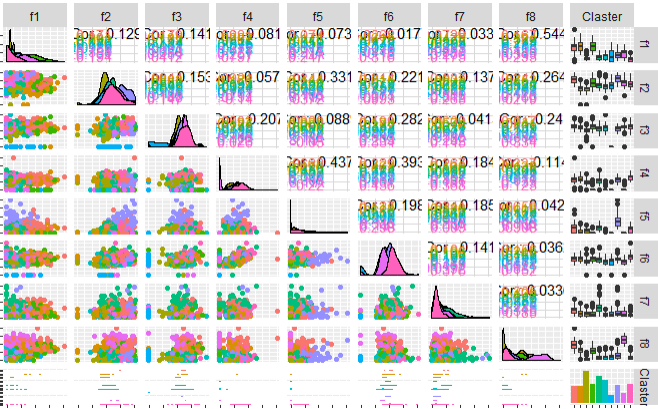
\includegraphics[width=1\textwidth]{diabetesP10.PNG}
\caption{Podział na dziesięć klastrów}
\end{figure}

\section{Analiza zbioru data knowledge modeling}
Zbiór knowledge zawiera realne dane dotyczące wiedzy stduentów o maszynach napędzanych silnikiem prądu stałego. Zawiera pięć atrybutów:
\textbf{STG} Stopień czasu nauki poświęconego na osiągnięcie celu materiałów\\
\textbf{SCG} Stopień powtarzania materiału\\
\textbf{STR} Stopień czasu poświęconego na studiowanie zagadnień związanych z tematem\\
\textbf{LPR} Ocena egzaminacyjna studenta odnośnie zagadnień związanych z tematem\\
\textbf{PEG} Ocena egzaminacyjna wiedzy zdobytej na dany temat\\

Obiektom przypisana została dyskretna wartość oceny, która przez skrypt jest tłumaczona na czterostopniową skalę (1-very low, 2-low, 3-medium, 4-high).

\begin{figure}[H]
\centering
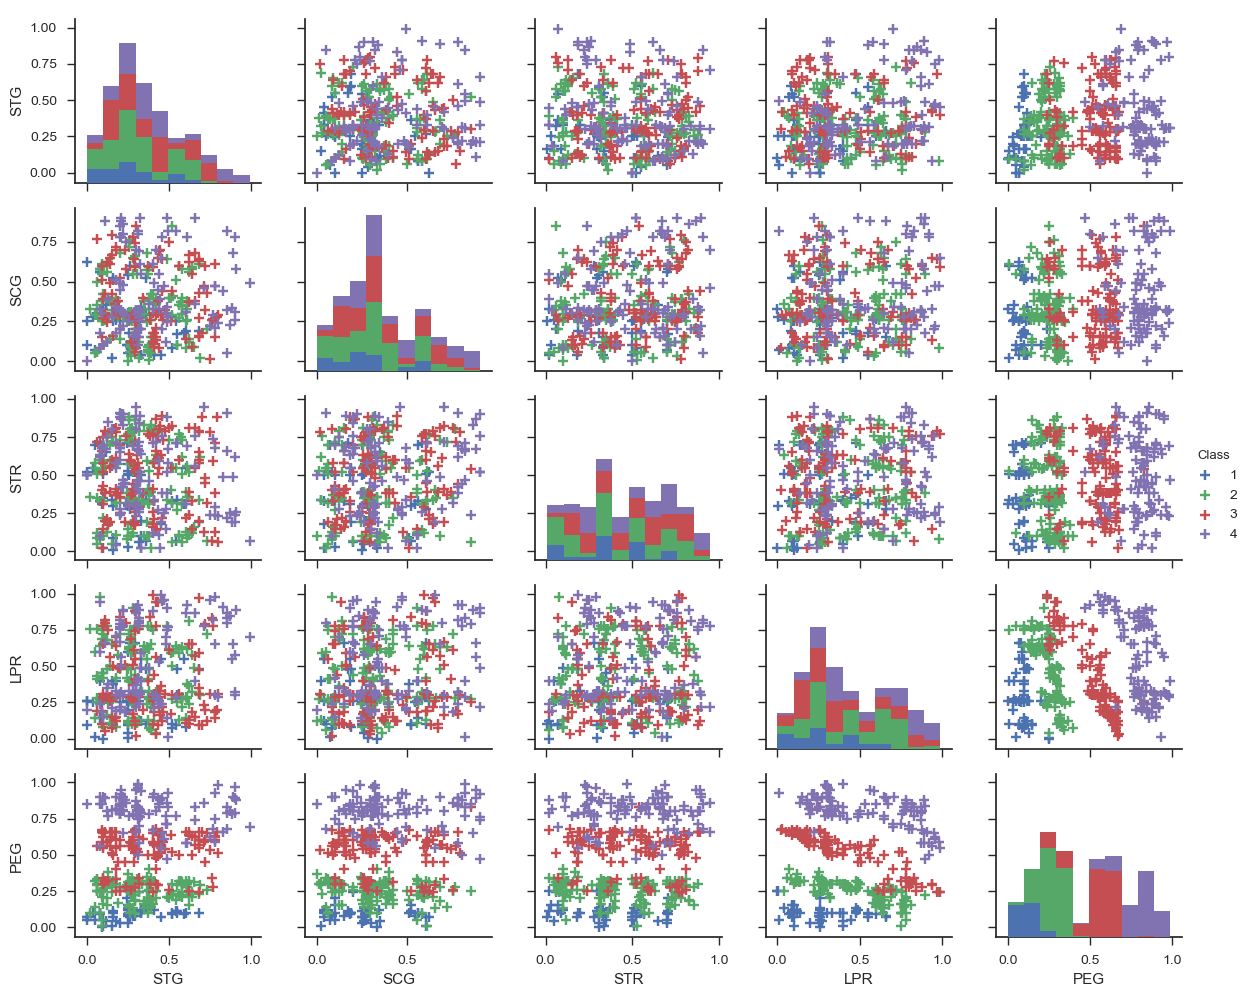
\includegraphics[width=1\textwidth]{dsKnowledgeCombined.png}
\caption{Rozkład cech dla zbioru Knowledge}
\end{figure}

Analiza wszystkich atrybutów do klasteryzacji została przeanalizowan w poprzednim rozdziale. Widać jednak, że pod kątem klas najlepsze rozróżnienie niesie para atrybutów LPR, PEG. Przy podziale na około 12 klastrów, wokół których skupiać będą się grupy powinniśmy otrzymać zadowalające wyniki.

\begin{figure}[H]
\centering
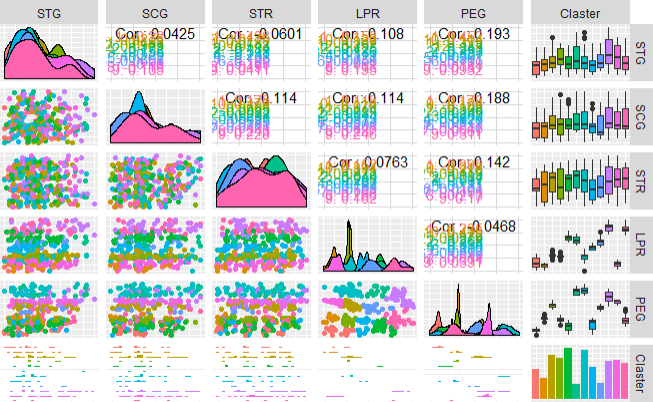
\includegraphics[width=1\textwidth]{selectedFeaturesKnowledge.PNG}
\caption{Rozkład cech dla zbioru Knowledge przy 12 klastrach i wyborze parametrów (PEG, LPR)}
\end{figure}

\begin{tabular}{ |p{2.5cm}||p{2.5cm}|p{2.5cm}|p{2.5cm}|p{2.5cm}| }

\hline
\multicolumn{5}{|c|}{Knowledge - statystyki}\\
\hline
context &Purity & Rand Index & Dunn Index & DBI \\
\hline
All & 0.896 & 0.788 & 0.065 & 3.443\\
Features & 0.896 & 0.788 & 0.045 & 0.780\\
\hline
\end{tabular}

\vspace{1cm}

Wskaźniki zewnętrzne, które są powiązane z przynależnością do konkretnych klas uległy znaczącej poprawie. Natomiast w przypadku wskaźników wewnętrznych widać, że w kontekście wszystkich atrybutów, wielkość klastrów znacząco wzrosła.

\section{Wnioski}
Klasteryzacja to potężne narzędzie pomagające nam przyporządkowywać obiekty do grup wyznaczonych na podstawie cech. Po powiązaniu otrzymanych grup z cechami możemy wykorzystać tą wiedzę do zadania klasyfikacji. Warto jednak dogłębnie zaznajomić się ze zbiorami, ponieważ uwzględnianie wszystkich atrybutów nie koniecznie wiąże się z poprawą jakości klasteryzacji.
\end{document}
